\documentclass[12pt, a4paper]{article}
\usepackage{graphicx}
\usepackage{pgfplots}
\usepackage{mathtools}
\usepackage{fancyhdr}
\usepackage{multicol}
\usepackage{cancel}
\usepackage{geometry}
\usepackage{listings}
\usepackage{booktabs}
\usepackage{tabularx}
\usepackage{subfig}
\usepackage{hyperref}
\usepackage{float}
\usepackage{titlesec}
\usepackage{tikz, pgfplots}
\usepackage[utf8]{inputenc}
\usepackage[backend=bibtex8,style=ieee]{biblatex}

% Requirement libs
\usetikzlibrary{positioning}

% Options
\nonstopmode % To make sure that you dont have to press input for each error
\geometry{top=1in, left = 1in, right = 1in, bottom=1.2in}
\pgfplotsset{compat=1.18}
\graphicspath{{./figures/}}
\setlength{\columnsep}{0.7cm}

% Metadata
\addbibresource{./citations.bib}
\author{Aris Podotas}
\date{today}

% Herlink setup
\hypersetup{
    colorlinks=true,
    linkcolor=blue,
    filecolor=magenta,
    urlcolor=cyan,
    pdftitle={MLICB Assignment 1},
    pdfpagemode=FullScreen,
}

% For the code blocks
\definecolor{codegreen}{rgb}{0.03,0.5,0.03}
\definecolor{codegray}{rgb}{0.5,0.5,0.5}
\definecolor{codepurple}{rgb}{0.58,0,0.82}
\definecolor{backcolour}{rgb}{0.95,0.95,0.95}

% Code block setup
\lstdefinestyle{mystyle}{
    backgroundcolor=\color{backcolour},
    commentstyle=\color{codegreen},
    keywordstyle=\color{magenta},
    numberstyle=\tiny\color{codegray},
    stringstyle=\color{codepurple},
    basicstyle=\ttfamily\footnotesize,
    breakatwhitespace=false,
    breaklines=true,
    captionpos=b,
    keepspaces=true,
    numbers=left,
    numbersep=5pt,
    showspaces=false,
    showstringspaces=false,
    showtabs=false,
    tabsize=4,
    escapeinside = {(*}{*)}
}
\lstset{style=mystyle}

% My custom headers and margins 
\pagestyle{fancy}
\setlength{\headheight}{44pt}
\setlength{\headsep}{18pt}
\lhead{\includegraphics[scale = 0.2]{~/Documents/Masters/bnw unit.png}}
\chead{\quad Data Science and Information Technologies Master’s
National and Kapodistrian University of Athens}
\rhead{}
\lfoot{}
\cfoot{\thepage}
\rfoot{}

% Start
\begin{document}

% Custom title page
\begin{titlepage}
    \centering
    {\huge \textbf{Assignment 2}\par}
    \vspace{0.5cm}
    {\Large \textbf{Name:} Aris Podotas\par}
    \vspace{0.5cm}
    {\large \textbf{University:} National and Kapodistrian University of Athens\par}
    \vspace{0.5cm}
    {\large \textbf{Program:} Data Science and Information Technologies\par}
    \vspace{0.5cm}
    {\large \textbf{Specialization:} Bioinformatics - Biomedical Data\par}
    \vspace{0.5cm}
    {\large \textbf{Lesson:} Image Processing \& analysis \par}
    \vspace{0.5cm}
    {\large \textbf{Date:} May 2025\par}
    \tableofcontents
\end{titlepage}

\begin{multicols}{2}

    \section{Exercise 1} \label{sec:ex1}

    The function is a step function that increases the output values by a variable amount with step $30$. The minimum intensity is $10$ and the maximum is $200$ which is less than the input range on both ends. This should generally dim the image to some degree. Let us compare this function to one that does not alter the image.
    \newline

\end{multicols}

\begin{figure}[H]
    \begin{center}
        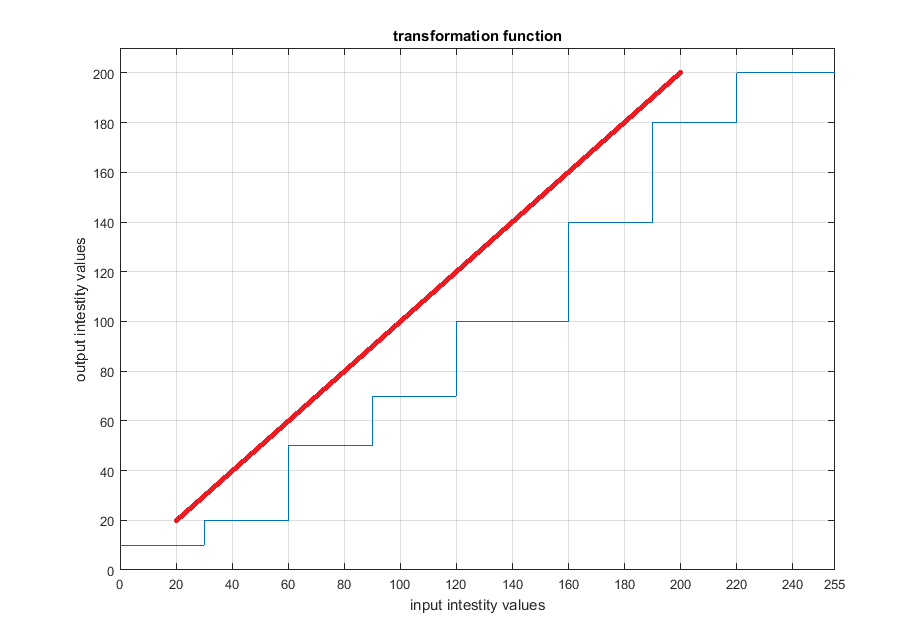
\includegraphics[width=0.95\textwidth]{figures/step_fun_vs_y_eq_x.png}
    \end{center}
    \caption{Comparison of the given function to one that does not alter the image (in red)}\label{fig:funcCompare}
\end{figure}

\begin{multicols}{2}

    Here we can see the dimming effect considering the step function is \textit{almost} always under the $y = x$ function that does not alter the image.
    \newline

    Since the function assigns an input range to a singular value we can expect some quantization of the output images. This should leave the output looking like a lower quality image and it will also be easier to compress but it will also be the same resolution right after the transformation.
    \newline

    \subsection{Example} \label{subsec:example}

    You can find the files that perform this transformation \href{https://github.com/ArisPodotas/Image-Processing-EX1/blob/master/src/req1.py}{here}.
    \newline

\end{multicols}

\begin{figure}[H]
    \begin{center}
        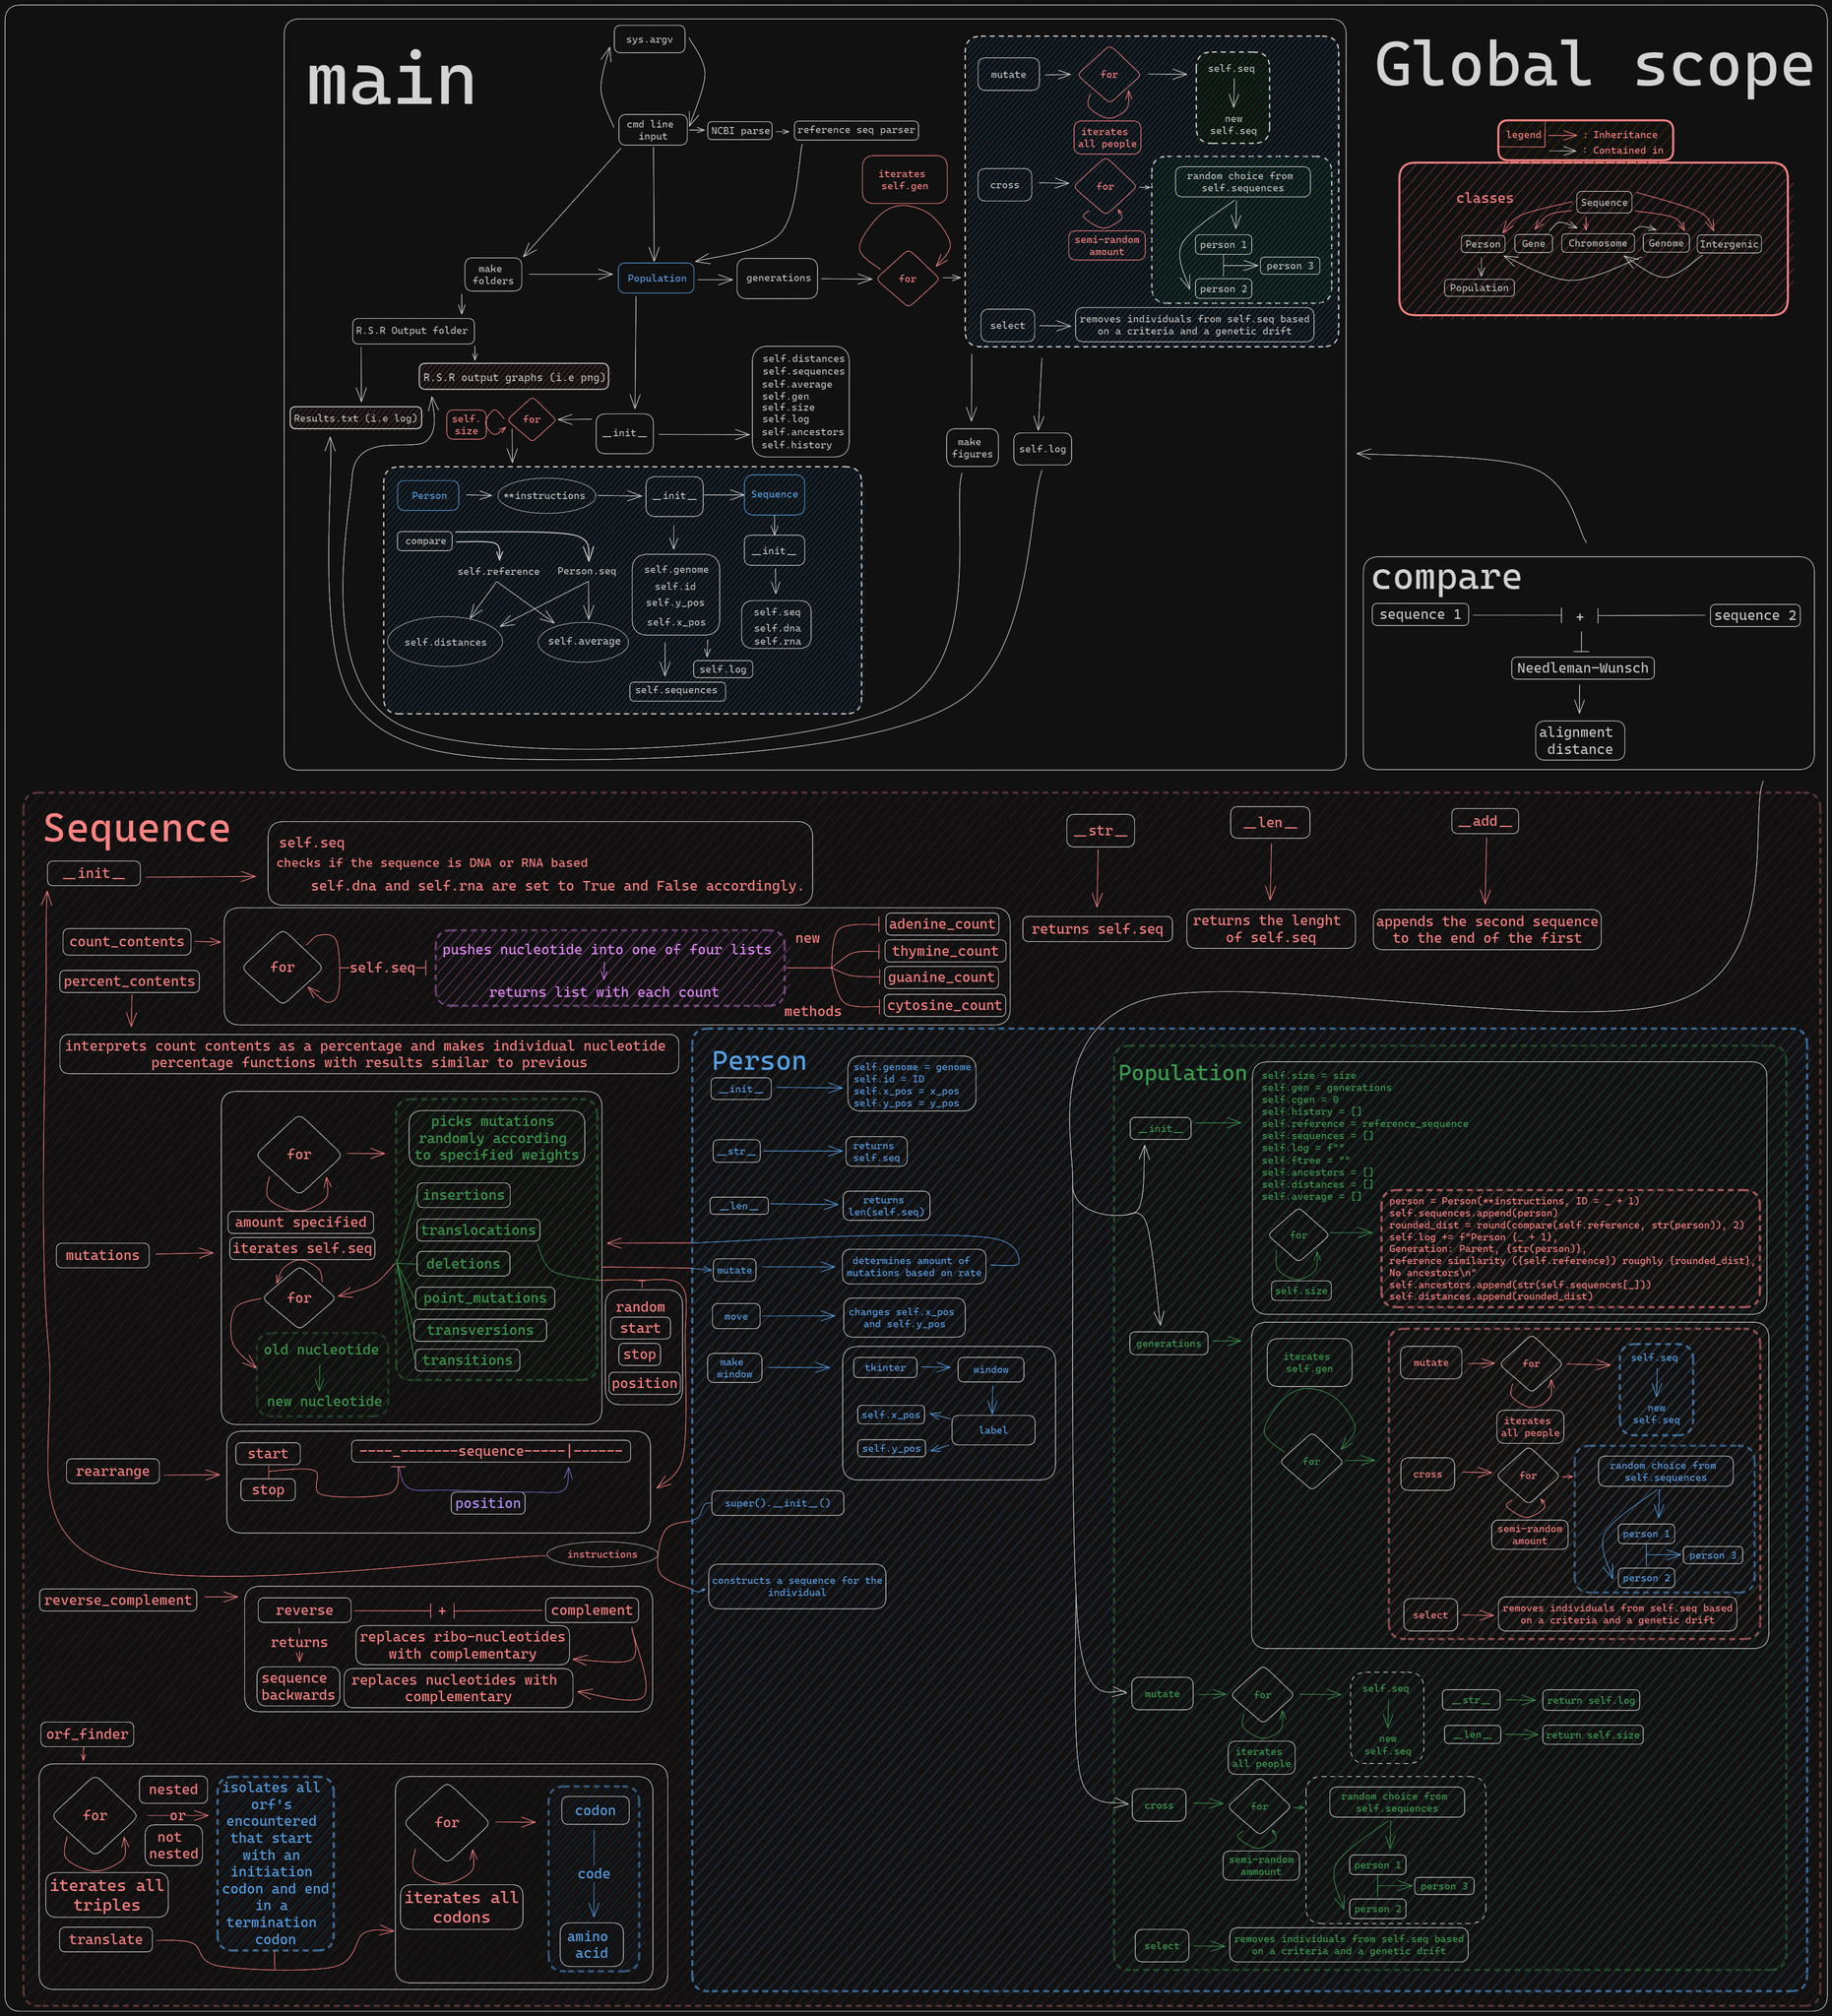
\includegraphics[width=0.95\textwidth]{figures/req1b.png}
    \end{center}
    \caption{Our image before the transformation}\label{fig:before}
\end{figure}

\begin{figure}[H]
    \begin{center}
        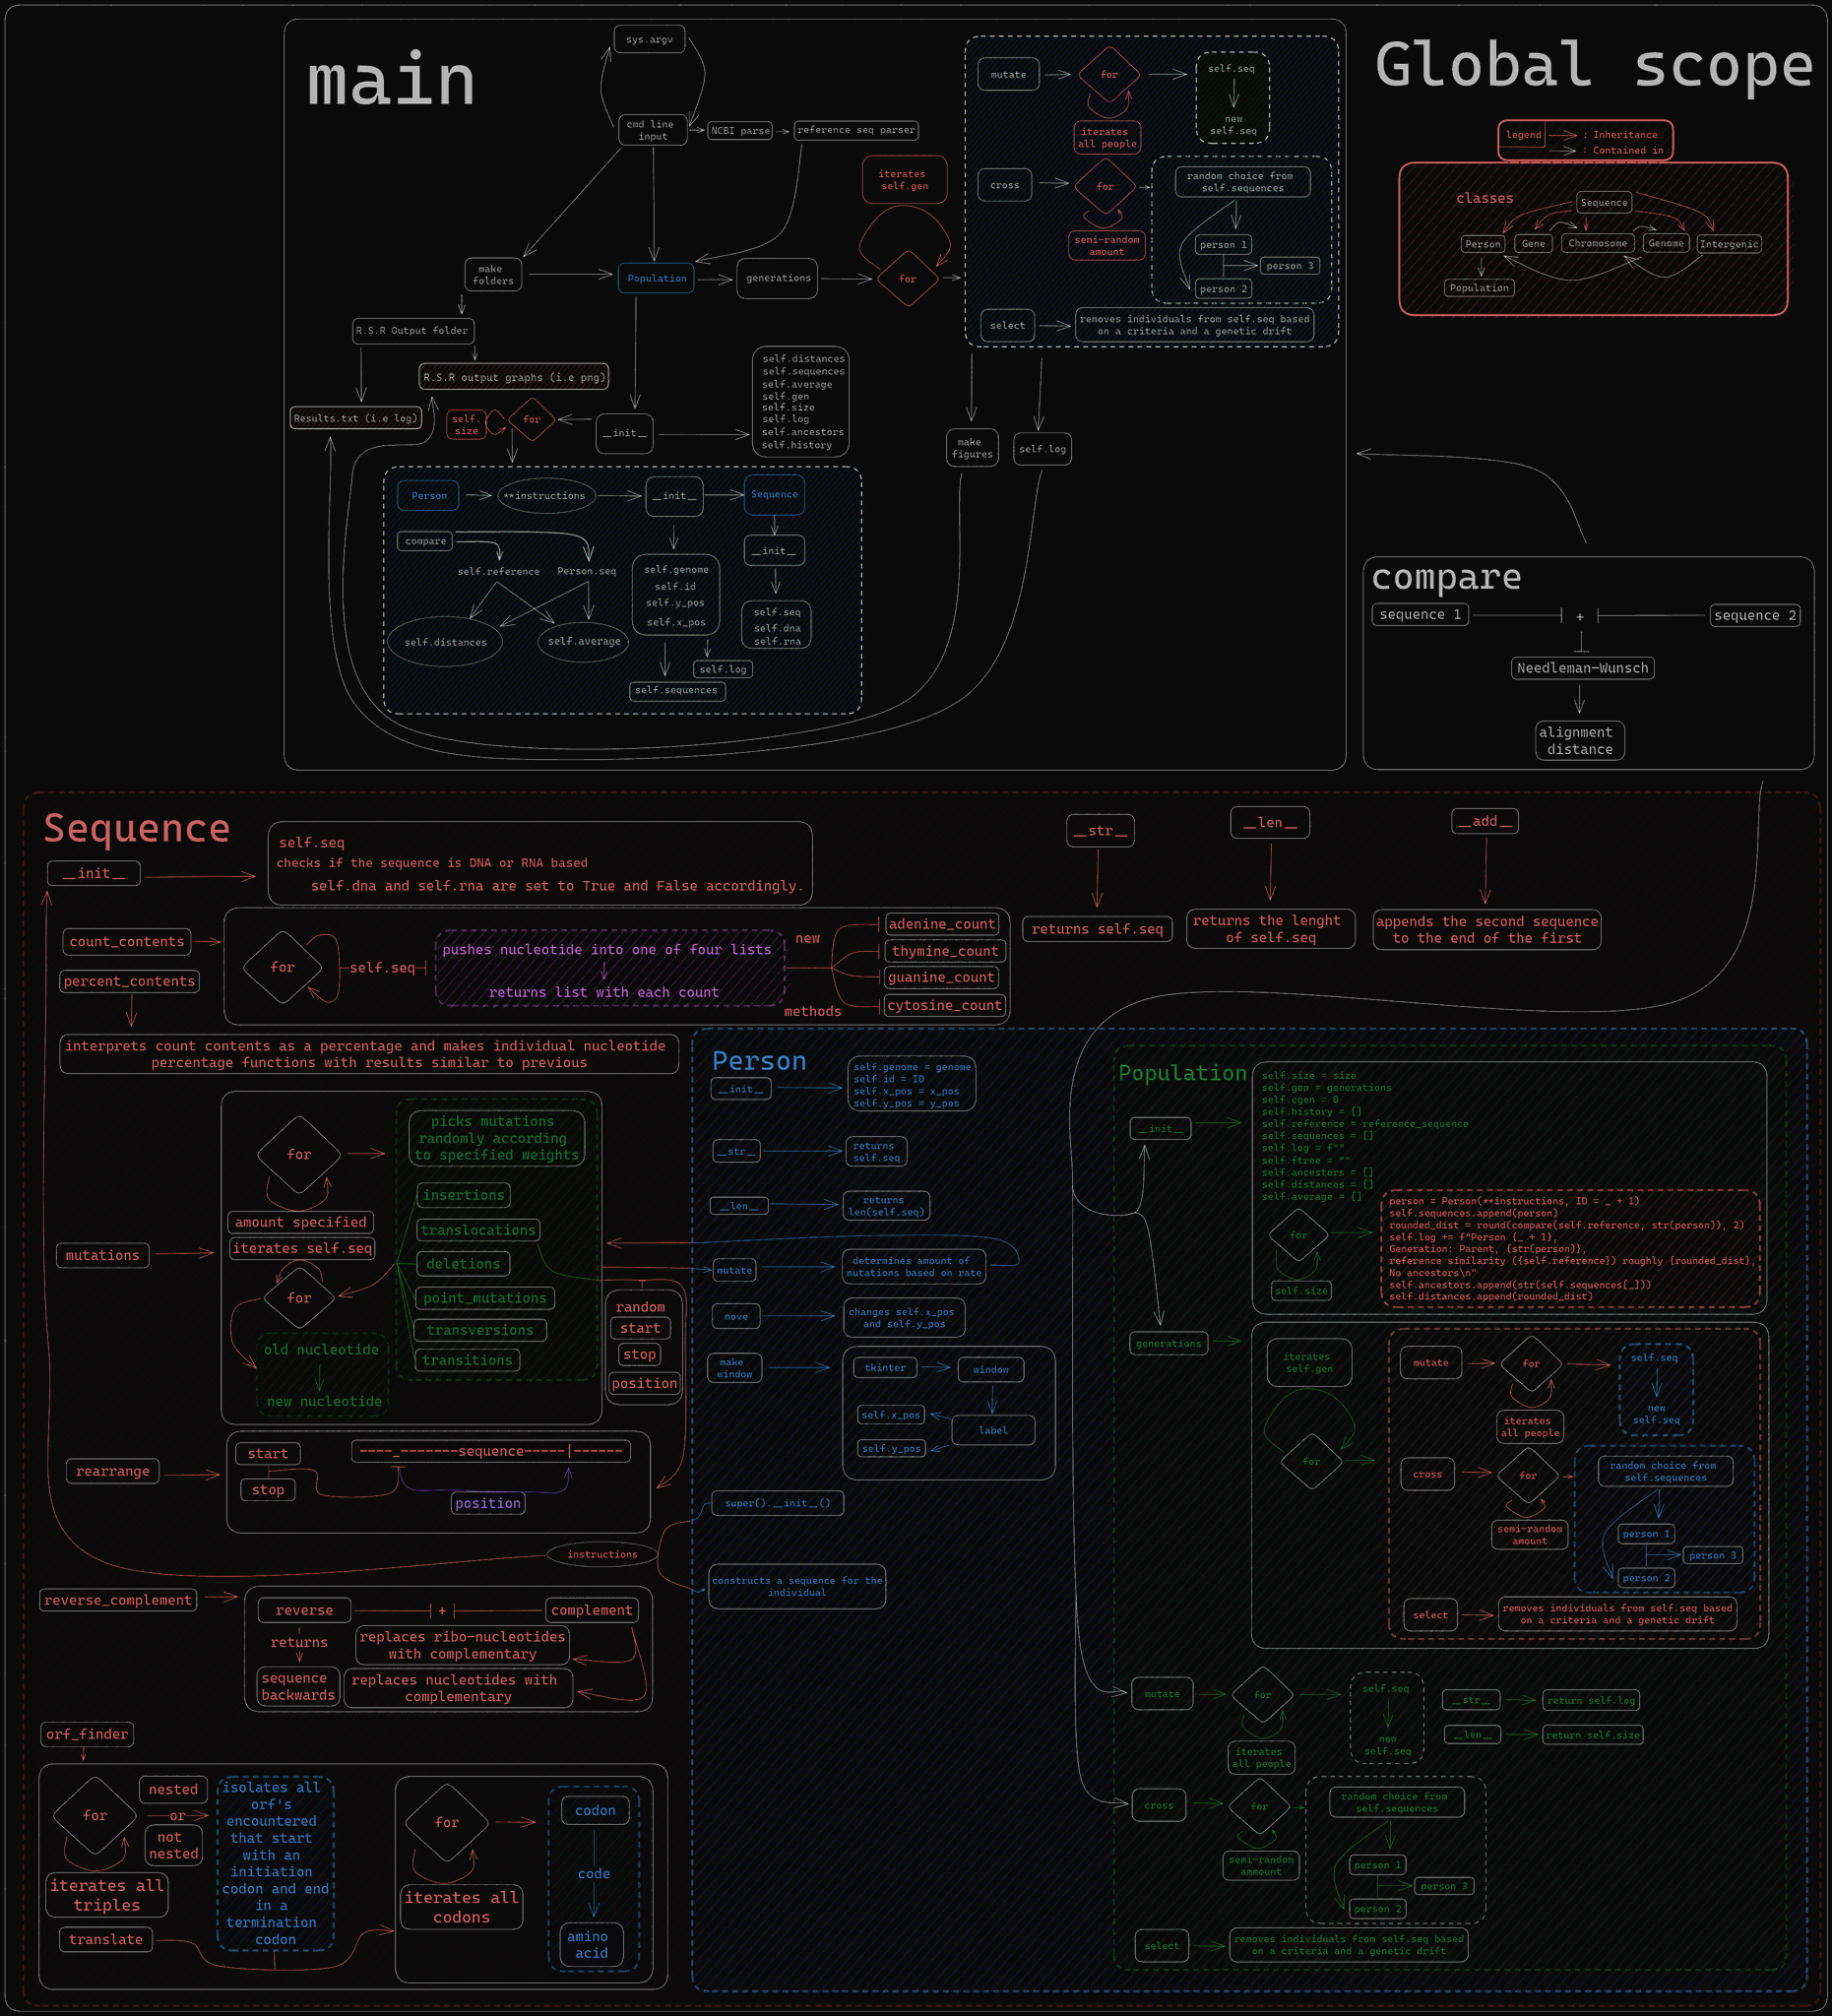
\includegraphics[width=0.95\textwidth]{figures/req1a.png}
    \end{center}
    \caption{Image after the transformation}\label{fig:after}
\end{figure}

\begin{multicols}{2}

    \begin{table}[H]
        \caption{Comparison of Images}\label{tab:comp}
        \begin{center}
            \resizebox{0.45 \textwidth}{!}{
                \begin{tabular}[c]{l|l|l|}
                    \hline
                    \multicolumn{1}{c|}{\textbf{Image}} & 
                    \multicolumn{1}{c}{\textbf{File Size (disk)}} &
                    \multicolumn{1}{c}{\textbf{Shape}} \\
                    \hline
                    Before & $3.29$ MB & $1861 \times 2048$ \\
                    After & $652$ KB & $1861 \times 2048$ \\
                    \hline
                \end{tabular}
            }
        \end{center}
    \end{table}

    We can see the quantization into a lower quality image while maintaining the same dimensions but a much lower disk space.
    \newline

    \section{Exercise 2} \label{sec:ex2}

    A gamma correction with a $G$ of more than 1 would lighten the image in the perception of the human eye.
    \newline

    \section{Exercise 3} \label{sec:ex3}

    The requirement says "a method" implying one but multiple transformations can be assigned to one method.
    \newline

    \begin{table}[H]
        \caption{Method Proposals}\label{tab:proposals3}
        \begin{center}
            \resizebox{0.45 \textwidth}{!}{
                \begin{tabular}[c]{l|l|}
                    \hline
                    \multicolumn{1}{c|}{\textbf{Method}} & 
                    \multicolumn{1}{c}{\textbf{Goal}} \\
                    \hline
                    Gamma correction & Accommodating for the perception of the human eye \\
                    Adding a constant & To bring up every pixels brightness \\
                    Multiplying by a constant & To bring up every pixels brightness \\
                    \hline
                \end{tabular}
            }
        \end{center}
    \end{table}

    Any one of the proposals or a combination of them would make the image appear brighter.
    \newline

    \section{Exercise 4} \label{sec:ex4}

    Taking a look at the image we can assume a median filter would not be suited to sharpening this image considering the edges and smooth regions, we should use some transformation that enhances the edges of the image. If we took the Laplacian of the image and used the isolated edges to alter only those pixels in the original image we would effectively increase the contrast of the edges and make the image look sharper. The proposal is to apply a gamma filter only to the pixels of the image that the Laplacian isolates ($G \geq 1$ ideally).
    \newline

    \section{Exercise 5} \label{sec:ex5}

    Lets look at some of the descriptive values for both images with our visual overview
    \newline

    \begin{table}[H]
        \caption{Comparison of Image\_1 and Image\_2}\label{tab:comparison}
        \begin{center}
            \resizebox{0.45 \textwidth}{!}{
                \begin{tabular}[c]{l|l|}
                    \hline
                    \multicolumn{1}{c|}{\textbf{Image}} & 
                    \multicolumn{1}{c}{\textbf{Size}} \\
                    \hline
                    Image\_1 & $800 \times 641$ \\
                    Image\_2 & $800 \times 641$ \\
                    \hline
                \end{tabular}
            }
        \end{center}
    \end{table}

    Visually it seems like we have just taken the negative of the image and since the scale of the image and the what side the aspects of the image are on has not changed we can assume a negative transformation has occurred. Upon zooming in we can see that Image\_2 has some quality nuance, but we can simply examine Image\_1 to see that it has this effect as well.
    \newline

    So the steps taken are those of getting the negative of an image which is to: 
    \newline

    \[f(x) = 255 - x\]
    \newline

    In order to do the opposite we need a function (let's call it $g(x)$) such that:
    \newline

    \[
        \resizebox{0.45\textwidth}{!}{$
        \begin{aligned}
            & g(f(x)) = x \iff g(255 - x) = x \iff \\
            & g(x) = f(x) = 255 - x
        \end{aligned}
        $}
    \]
    \newline

    \section{Exercise 6} \label{sec:ex6}

    Before any of the following, you will be able to find all source files in \href{https://github.com/ArisPodotas/Image-Processing-EX1/tree/master}{this repository}.
    \newline

    \section{Exercise 7} \label{sec:ex7}

    \printbibliography

\end{multicols}

\end{document}

